\documentclass{poly}
\usepackage{main}

\title{Chapitre 1 : Étude de fonctions polynomiales du second degré}
\date{}
\author{Premières Spécialité Mathématiques}

\begin{document}
\maketitle
\section{Rappel : Fonctions affines}
\begin{definition}
Une \textbf{fonction affine} est une fonction $f$ définie sur $\R$ telle que pour tout $x \in \R$ :
\begin{equation*}
f(x) = ax + b
\end{equation*}
avec $a \neq 0$ et $b$ deux réels.

Le réel $a$ est appelé \textbf{coefficient directeur} de $f$.

Le réel $b$ est appelé \textbf{ordonnée à l'origine} de $f$.
\end{definition}
\begin{remark}
Quand $b = 0$, c'est-à-dire quand $f(x) = ax$, on dit que la fonction est \textbf{linéaire}.
\end{remark}
\begin{proposition}
Soit $f : x \mapsto ax + b$ une fonction affine avec $a \neq 0$ et $b$ deux nombres réels; et $(O;I;J)$ un repère orthonormée. Alors, la courbe représentative de $f$ dans ce repère est une droite.
\end{proposition}
\begin{proposition}
Soit $(O;I;J)$ un repère orthonormée, et $f$ une fonction définie sur $\R$ dont la courbe représentative est une droite. Alors, $f$ est une fonction affine telle que $f(x) = ax + b$ pour tout $x \in \R$ où :
\begin{itemize}
\item son coefficient directeur $a$ est donnée par la pente de la droite;
\item son ordonnée à l'origine $b$ est l'ordonnée du point de la droite d'abscisse $0$.
\end{itemize}
\end{proposition}
\newpage
\begin{exercize}
\label{ex:affine}
Sur le repère $(0;I;J)$ ci-contre, on a tracé la courbe représentative de deux fonctions affines $f$ et $g$.
\begin{center}
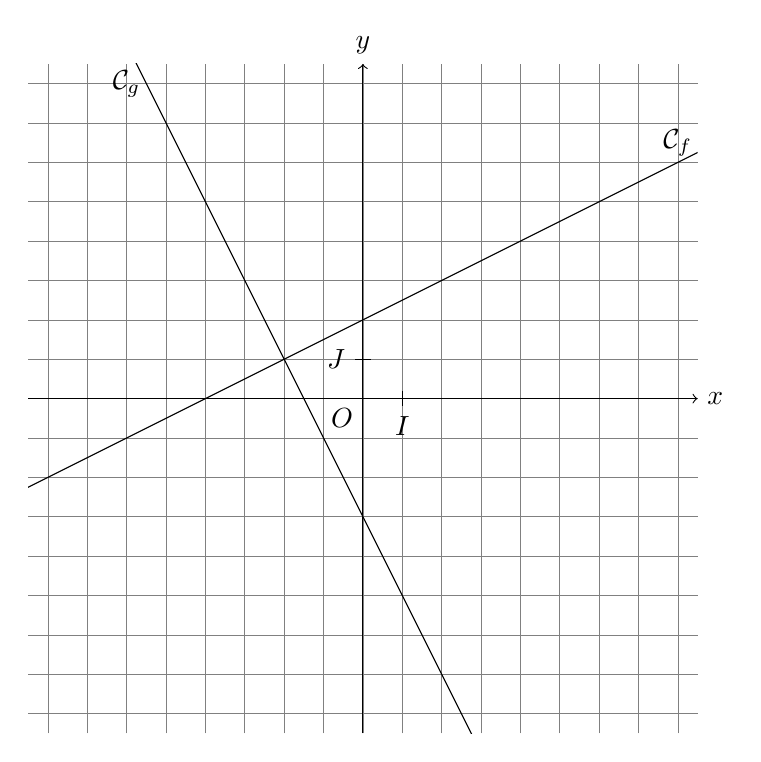
\begin{tikzpicture}
\draw[help lines] (-4.25,-4.25) grid[step=0.5] (4.25,4.25);
\draw[->] (-4.25,0) -- (4.25,0) node[right] {$x$};
\draw[->] (0,-4.25) -- (0,4.25) node[above] {$y$};
\draw (0,0) node[below left] {$O$};
\draw (0.5,0.1) -- (0.5,-0.1) node[below] {$I$};
\draw (0.1,0.5) -- (-0.1,0.5) node[left] {$J$};
\clip (-4.25,-4.25) rectangle (4.25,4.25);
\draw (-5,-1.5) -- (5,3.5);
\draw (-5,8.5) -- (5,-11.5);
\draw (4,3.25) node {$\mathcal{C}_f$};
\draw (-3,4) node {$\mathcal{C}_g$};
\end{tikzpicture}
\end{center}
En déduire l'expression algébrique de $f$ et $g$.
\end{exercize}
\begin{proposition}
Soit $f : x \mapsto ax + b$ une fonction affine, et $x_1 < x_2$ deux réels distincts. Alors,

\noindent\begin{minipage}{0.5\textwidth}
\begin{equation*}
a = \dfrac{f(x_2) - f(x_1)}{x_2 - x_1}
\end{equation*}
\end{minipage}
et
\begin{minipage}{0.5\textwidth}
\begin{equation*}
b = f(x_1) - ax_1
\end{equation*}
\end{minipage}
\end{proposition}
\begin{proposition}
Soit $f : x \mapsto ax + b$ une fonction affine.
\begin{itemize}
\item Si $a < 0$, alors $f$ est décroissante sur $\R$. 
\item Si $a > 0$, alors $f$ est croissante sur $\R$. 
\end{itemize}
\end{proposition}
\begin{method}
Pour dresser le tableau de signes d'une fonction affine $f : x \mapsto ax + b$, il faut:
\begin{enumerate}
\item Déterminer l'antécédant de $0$ de $f$, autrement dit, trouver $x$ tel que $ax + b = 0$;
\item Le tableau de signes s'obtient en suivant la variation de la fonction, autrement dit, cela dépend du signe de $a$ 
\end{enumerate} 
\end{method}
\begin{exercize}
Dresser le tableau de signes des fonctions trouvées dans l'exercice \ref{ex:affine}.
\end{exercize}

\newpage
\section{Fonction polynomiale du second degré}

\begin{definition}
Une \textbf{fonction polynomiale du second degré} est une fonction $f$ définie sur les réels qui à tout nombre $x$ associe un réel $f(x)$ de la forme:
\begin{equation*}
ax^2+bx+c   
\end{equation*}
où $a$, $b$ et $c$ sont des réels avec $a \neq 0$. 
\end{definition}

\begin{remark}
L'hypothèse $a \neq 0$ est essentielle, sinon la fonction est polynomiale de degré au plus $1$.    
\end{remark}

On trace la courbe représentative de deux fonctions polynomiales du second degré : une avec $a > 0$ et une avec $a < 0$.

\begin{minipage}{0.45\textwidth}
\begin{center}
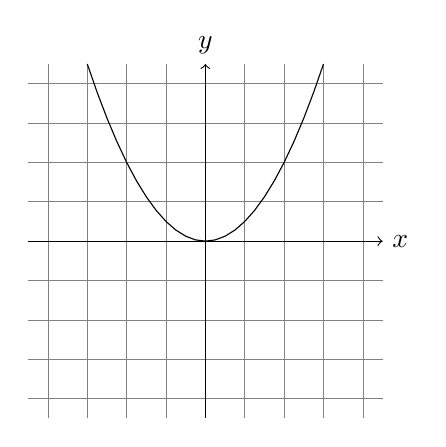
\begin{tikzpicture}
\draw[help lines] (-2.25,-2.25) grid[step=0.5] (2.25,2.25);
\draw[->] (-2.25,0) -- (2.25,0) node[right] {$x$};
\draw[->] (0,-2.25) -- (0,2.25) node[above] {$y$};
\draw[domain=-1.5:1.5] plot (\x, \x*\x);
\end{tikzpicture}
\end{center}   
\end{minipage}
\hfill
\begin{minipage}{0.45\textwidth}
\begin{center}
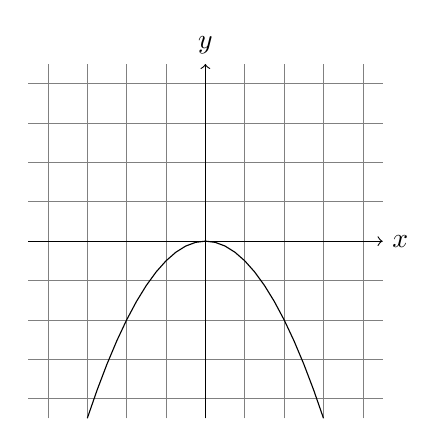
\begin{tikzpicture}
\draw[help lines] (-2.25,-2.25) grid[step=0.5] (2.25,2.25);
\draw[domain=-1.5:1.5] plot (\x, -\x*\x);
\draw[->] (-2.25,0) -- (2.25,0) node[right] {$x$};
\draw[->] (0,-2.25) -- (0,2.25) node[above] {$y$};
\end{tikzpicture}
\end{center}    
\end{minipage}
\vspace*{0.5cm}
\begin{definition}
Soit $f$ une fonction polynomiale de degré $2$. Sa courbe représentative est appelée une \textbf{parabole}.
\end{definition}
\begin{proposition}
Soit $f$ une fonction polynomiale de degré $2$. telle que $f(x) = ax^2 + bx + c$. Alors:
\begin{itemize}
\item Si $a > 0$, il existe une valeur de $x$, notée $x_m$ telle que $f$ est décroissante sur $\left] - \infty; x_m \right]$ et croissante sur $\left[x_m; + \infty \right[$
\item Si $a < 0$, il existe une valeur de $x$, notée $x_M$ telle que $f$ est croissante sur $\left] - \infty; x_M \right]$ et décroissante sur $\left[x_M; + \infty \right[$
\end{itemize}
\end{proposition}
\begin{remark}
\hfill
\begin{itemize}
\item Dans le cas $a > 0$, les \emph{\og branches de la paraboles sont tournées vers le haut \fg}. Dans le cas contraire ($a < 0$), elles sont \emph{\og tournées vers le bas \fg}.
\item Dans le cas $a > 0$, $f$ admet un unique minimum, et ce minimum est atteint en $x_m$. Dans le cas contraire ($a < 0$), $f$ admet un maximum, et ce maximum est atteint en $x_M$. 
\end{itemize}
\end{remark}
\newpage
\section{Recherche de l'extremum}
\subsection{Forme canonique}
\begin{proposition}
Soit $f$ une fonction polynomiale du second degré telle que $f(x) = ax^2 + bx + c$. Alors il existe $\alpha$ et $\beta$ tel que
\begin{equation*}
f(x) = a(x - \alpha)^2 + \beta
\end{equation*}
\end{proposition}

\begin{remark}
Dans ce cas, $\alpha = \dfrac{-b}{2a}$ et $\beta = f(\alpha)$.
\end{remark}
\begin{example}
Soit l'expression polynomiale du second degré $- x^2 + 2x - 5$. Déterminer sa forme canonique.

\begin{method}[Par identification]
\end{method}    
\begin{method}[En utilisant les développements limités]
\end{method}
\end{example}
\newpage
\subsection{Extremum}   
\begin{proposition}
Soit une fonction polynomiale du second degré $f : x \mapsto ax^2 + bx + c$. On suppose que $f(x) = a(x - \alpha)^2 + \beta$ pour tout $x$ réel. Alors, $f$ admet un extremum qu'il atteint en $\alpha$ et ayant pour valeur $\beta$.    
\end{proposition}
\begin{remark}
Comme dit précédemment, si $a > 0$, alors $f$ admet un minimum qu'il attent en $\alpha = \dfrac{-b}{2a}$. Sinon, si $a < 0$, alors $f$ admet un maximum qu'il atteint en $\alpha = \dfrac{-b}{2a}$. Dans les deux cas, cet extremum vaut $\beta = f(\alpha)$.
\end{remark}
\begin{example}
Soit la fonction polynomiale $g : x \mapsto 4x^2 + 32x - 5$.
\begin{alphaquestions}
\item Cette fonction admet-elle un minimum ou un maximum ?
\item En quelle valeur cet extremum est-il atteint ?
\item Que vaut cet extremum ?
\end{alphaquestions}
\end{example}
\begin{proposition}
Soit $f : x \mapsto ax^2 + bx + c$ une fonction polynomiale du second degré. On suppose que $f(x) = a(x - \alpha)^2 + \beta$. Alors la courbe représentative $\mathcal{C}_f$ est une parabole admettant comme axe de symétrie la droite $x = \alpha$.
\end{proposition}
\begin{example}
Soit $f : x \mapsto x^2 - 2x + 1$. Alors $f$ admet un minimum (car $a > 0$) atteint en $\alpha = - \dfrac{b}{2a} = - \dfrac{-2}{2} = 1$. Alors $\mathcal{C}_f$ admet la droite $x = 1$ comme axe de symétrie.
\begin{center}
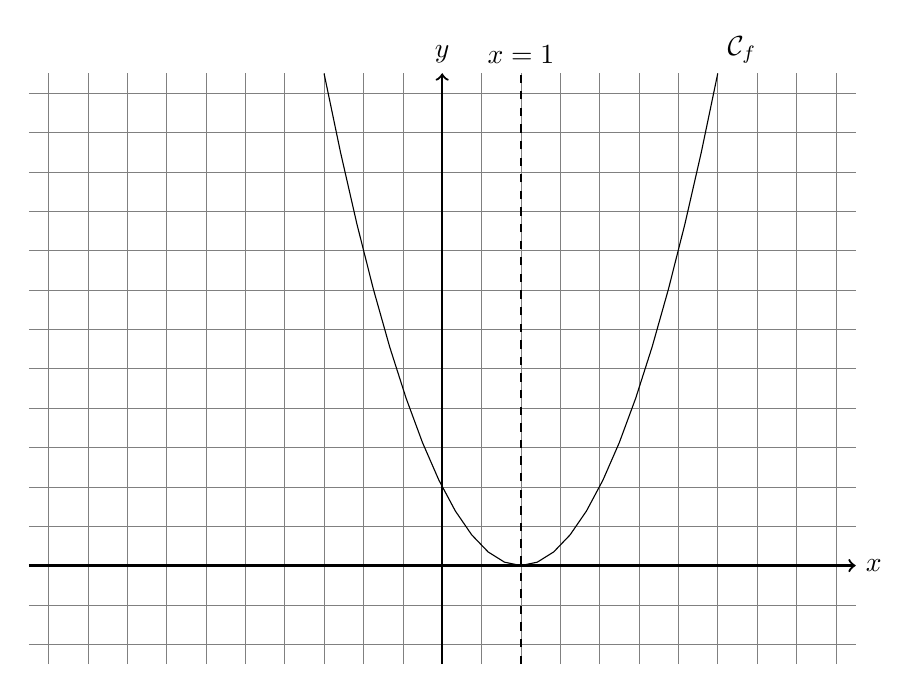
\begin{tikzpicture}
\draw[help lines] (-5.25,-1.25) grid[step=0.5] (5.25,6.25);
\draw[->,thick] (-5.25,0) -- (5.25,0) node[right] {$x$};
\draw[->,thick] (0,-1.25) -- (0,6.25) node[above] {$y$};
\draw plot[domain=-1.5:3.5] (\x, \x * \x - 2 * \x + 1) node[above right] {$\mathcal{C}_f$};
\draw[dashed,thick] (1,-1.25) -- (1,6.25) node[above] {$x = 1$};
\end{tikzpicture}
\end{center}
\end{example}

\newpage

\section{Racines}

\subsection{Définition}

\begin{tcolorbox}
\begin{definition}
Soit $f$ une fonction. On appelle \textbf{racine} de la fonction $f$ un nombre $r$ tel que $f(r) = 0$.
\end{definition}
\end{tcolorbox}
\begin{example}
Vérifier que $r_1 = 1$ et $r_2 = - 3$ sont deux racines de la fonction $f : x \mapsto 2x^2 + 4x - 6$.
\vspace*{0.2cm}

\end{example}
\begin{proposition}
Soit $f : ax^2 + bx + c$ une fonction polynomiale du second degré. Alors, seuls trois cas sont à considérer :
\begin{alphaquestions}
\item $f$ n'admet aucune racine réelle, c'est-à-dire que pour tout réel $x$, on a $f(x) \neq 0$.
\item $f$ admet une unique racine notée $r$. Dans ce cas, $f$ peut être factorisée en $f(x) = a (x - r)^2$ pour tout $x$.
\item $f$ admet deux racines, notées $r_1$ et $r_2$. Dans ce cas, $f$ peut être factorisée en $f(x) = a(x - r_1)(x - r_2)$ pour tout $x$.    
\end{alphaquestions} 
\end{proposition}
\begin{example}
Soient trois fonctions polynomiales du second degré $f$, $g$ et $h$, dont les courbes $\mathcal{C}_f$, $\mathcal{C}_g$ et $\mathcal{C}_h$ sont représentées ci-après. Combien de racines ont chacune de ces fonctions ?
\begin{center}
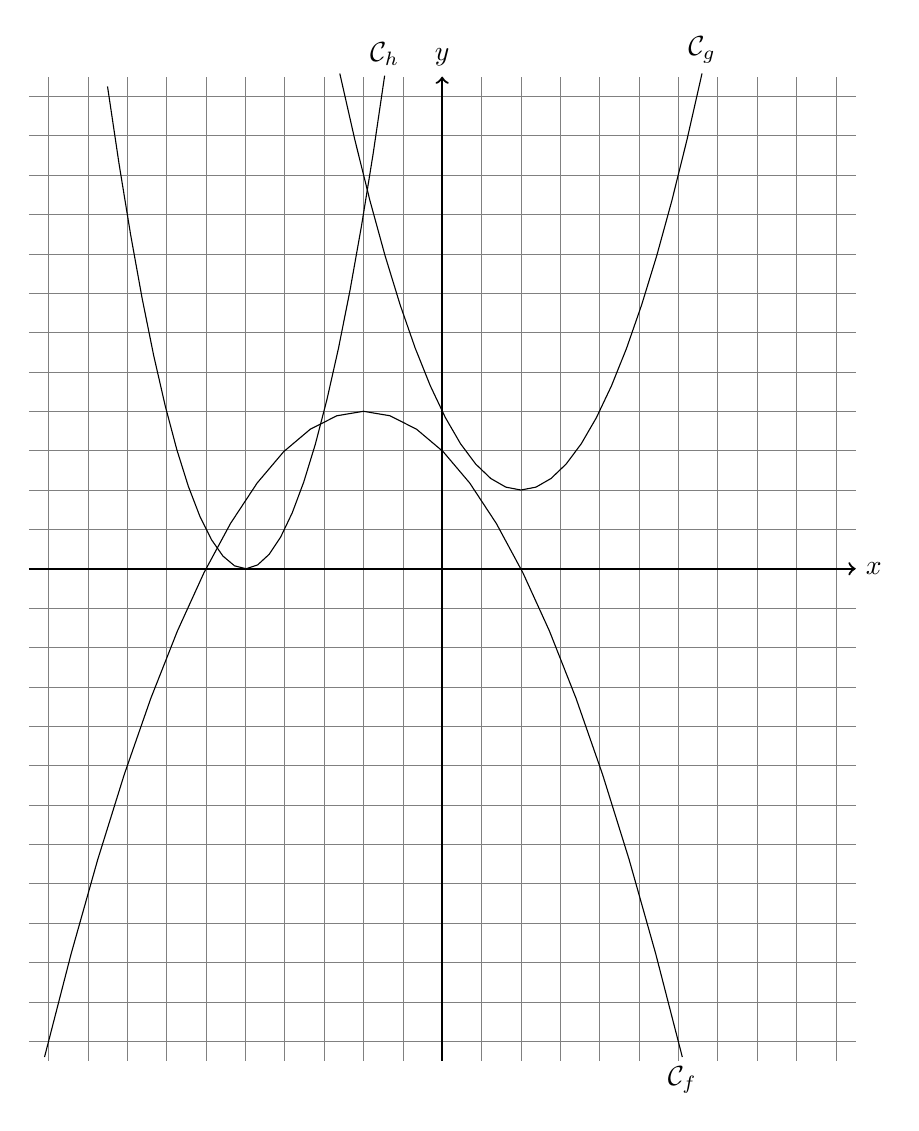
\begin{tikzpicture}
\newcommand{\Le}{-5.25};
\newcommand{\Ri}{5.25};
\newcommand{\To}{6.25};
\newcommand{\Bo}{-6.25};
\coordinate (LB) at (\Le,\Bo);
\coordinate (RT) at (\Ri,\To);
\draw[help lines] (LB) grid[step = 0.5] (RT);
\draw[thick,->] (\Le,0) -- (\Ri,0) node[right] {$x$};
\draw[thick,->] (0,\Bo) -- (0,\To) node[above] {$y$}; 
\draw[domain=-5.05:3.05] plot ({\x},{-0.5*(\x - 1)*(\x + 3)}) node[below] {$\mathcal{C}_f$}; 
\draw[domain=-1.3:3.3] plot ({\x},{(\x - 1)^2 + 1}) node[above] {$\mathcal{C}_g$};
\draw[domain=-4.25:-0.73] plot ({\x},{2*(\x + 2.5)^2}) node[above] {$\mathcal{C}_h$};
\end{tikzpicture}
\end{center}
\end{example}
\newpage
\subsection{Signe}
\begin{proposition}
Soit $f : x \mapsto ax^2 + bx + c$ une fonction polynomiale du second degré. Alors:
\begin{alphaquestions}
\item Si $f$ n'admet pas de racine, alors $f$ est du même signe que $a$ sur $\R$.
\item Si $f$ admet une unique racine $r$, alors $f$ est du même signe que $a$ sur $\left]-\infty;r\right[$ et sur $\left]r;+\infty\right[$.
\item Si $f$ admet deux racines distinctes $r_1 < r_2$, alors $f$ est du même signe que $a$ sur $\left]-\infty;r_1\right[$ et sur $\left]r_2;+\infty\right[$, et est du signe opposé à $a$ sur $\left]r_1;r_2\right[$
\end{alphaquestions}
\end{proposition}
\begin{remark}
Une phrase pour retenir cette proposition :
\begin{tcolorbox}
\begin{quote}
Une fonction polynomiale du second degré est du même signe que $a$ à \textbf{l'extérieur} de ses racines, et est de signe opposé à $a$ à \textbf{l'intérieur} de ses racines.
\end{quote}
\end{tcolorbox}
\end{remark}
\begin{example}
En reprenant l'exemple précédent, donner le tableau de signes des fonctions $f$, $g$ et $h$.
\end{example}
\subsection{Calcul des racines}
\subsubsection{En identifiant une racine évidente}
Soit $f(x) = -x^2 + 6x$ pour $x \in \R$. Alors, l'équation $f(x) = 0$ admet deux solutions évidentes : $0$ et $6$. Comme $f$ est une fonction polynomiale du second degré, alors on sait que ce sont les seules solutions réelles possibles.
\subsubsection{En utilisant une identité remarquable}
Soit $f(x)= 2x^2 - 128$ pour $x \in \R$. Alors, la troisième identité remarquable nous donne un factorisation de $f(x) = 2(x - 8)(x + 8)$. Donc les deux racines distinctes de la fonction polynomiale du second degré $f$ sont $8$ et $-8$.

\subsubsection{Avec le produit et la somme des racines}
\begin{proposition}
Soit $f : x \mapsto ax^2 + bx + c$ une fonction polynomiale du second degré. Si $r_1$ et $r_2$ sont les deux racines (possiblement confondues) de $f$, alors
\begin{equation*}
r_1 + r_2 = \dfrac{-b}{a} \qquad r_1 \times r_2 = \dfrac{c}{a}
\end{equation*}
\end{proposition}
\begin{example}
Soit $f(x) = x^2 + x - 20$. On remarque que $4$ est une racine de $f$. En déduire une autre racine de $f$, puis une factorisation de $f$.
\vspace*{0.5cm}

\end{example}
\newpage
\subsubsection{Avec le discriminant}
\begin{tcolorbox}
\begin{definition}
Soit $f : x \mapsto ax^2 + bx + c$ une fonction polynomiale du second degré. Alors on appelle \textbf{discriminant de f}, noté $\Delta$, la quantité
\begin{equation*}
\Delta = b^2 - 4ac
\end{equation*} 
\end{definition}
\end{tcolorbox}
\begin{theorem}
Soit $f : x \mapsto ax^2 + bx + c$ une fonction polynomiale de second degré, et $\Delta$ son discriminant. Alors:
\begin{alphaquestions}
\item Si $\Delta < 0$, alors $f$ n'admet pas de racine réelle.
\item Si $\Delta = 0$, alors $f$ admet une unique racine réelle $r$, telle que
\begin{equation*}
r = - \dfrac{b}{2a}
\end{equation*}
\item Si $\Delta > 0$, alors $f$ admet deux racines réelles distinctes $r_1 < r_2$, telles que
\begin{equation*}
r_1 = \dfrac{- b - \sqrt{\Delta}}{2a} \qquad r_2 = \dfrac{- b + \sqrt{\Delta}}{2a}
\end{equation*}
\end{alphaquestions}
\end{theorem}
\paragraph{Démonstration}
\hfill
\vspace*{0.2cm}

\end{document}